\documentclass{article}
\usepackage{arxiv}

\usepackage[utf8]{inputenc}
\usepackage[T1]{fontenc}
\usepackage{hyperref}
\usepackage{url}
\usepackage{booktabs}
\usepackage{amsfonts}
\usepackage{nicefrac}
\usepackage{microtype}
\usepackage{graphicx}
\usepackage{xcolor}
\usepackage{listings}
\usepackage{pgfplots}
\usepackage{multicol}

\pgfplotsset{compat=1.18}

\lstset{
  basicstyle=\ttfamily\small,
  breaklines=true,
  frame=single,
  framesep=3pt,
  columns=fullflexible,
  keepspaces=true,
  aboveskip=8pt,
  belowskip=8pt,
  xleftmargin=4pt,
  xrightmargin=4pt,
}

\title{AXI: Designing Ergonomic Interfaces for Autonomous Agents}

\author{
  Kun Chen \\
  \texttt{kun@kunchenguid.com}
}

\begin{document}
\maketitle

% ---------------------------------------------------------------------------
% ABSTRACT
% ---------------------------------------------------------------------------
\begin{abstract}
Autonomous AI agents interact with external services through two dominant
paradigms: shell-executed CLIs and structured tool protocols such as MCP.
Both impose significant overhead on agents---CLIs produce verbose,
metadata-sparse output that wastes token budgets, while MCP tool schemas
consume 3--4$\times$ more context tokens and 2--3$\times$ more cost per task.
This paper presents the Agent eXperience Interface (AXI), a set of 10 design
principles for building agent-facing CLIs that address both problems. AXI
introduces token-optimized output formatting, pre-computed aggregate fields,
contextual next-step suggestions, and structured error handling.
AXI is evaluated against four alternative interfaces---raw CLI, two MCP
configurations, and a code-generation approach---across 425 benchmark runs
(17 tasks $\times$ 5 conditions $\times$ 5 repeats) using Claude Sonnet~4.6.
AXI achieves 100\% task success at the lowest cost (\$0.050/task) and fastest
duration (15.7s), compared to 86\% at \$0.054 for raw CLI and 82--87\% at
\$0.101--0.148 for MCP conditions.
\end{abstract}

\keywords{AI agents \and tool use \and command-line interfaces \and benchmark \and LLM}

% ---------------------------------------------------------------------------
% 1  INTRODUCTION
% ---------------------------------------------------------------------------
\section{Introduction}
\label{sec:intro}

AI agents interact with external services through two dominant paradigms.
The first is \textbf{shell-based CLI execution}: the agent runs commands like
\texttt{gh issue list} and parses the text output. The second is
\textbf{structured tool protocols} like MCP (Model Context Protocol), where
the agent invokes typed tool functions through the hosting framework's native
tool-calling interface.

Both approaches have significant problems for agents:

\begin{itemize}
  \item \textbf{CLI: verbose, metadata-sparse output.} Human-oriented CLIs
    produce tab-separated tables, ANSI formatting, and per-item descriptions
    that waste token budget. Worse, they omit critical metadata---a label list
    returns 30 items with no total count, and the agent reports 30 when the
    actual answer is 126.
  \item \textbf{MCP: massive schema overhead.} MCP tool definitions consume
    137K--176K input tokens per task in this benchmark, compared to 46--47K for
    CLI conditions. This 3--4$\times$ context inflation translates directly to
    2--3$\times$ higher cost per task (\$0.10--0.15 vs.\ \$0.05).
  \item \textbf{Both: poor discoverability.} CLI agents must guess subcommands
    or read \texttt{-{}-help}. MCP agents with lazy loading waste turns on
    tool discovery. Neither provides in-context guidance on what to do next.
\end{itemize}

Recent debate has framed this as ``MCP vs.\ CLI''~\cite{smithery2026}, but
the real question is neither \emph{which} protocol nor \emph{which} transport,
but rather \emph{what design principles} make an agent-tool interface
effective. This paper proposes the \textbf{Agent eXperience Interface (AXI)}---10
principles for agent-facing CLI design that treat token budget as a
first-class constraint. AXI achieves the reliability advantages MCP promises
(structured output, discoverability) at the cost profile of a CLI.

Contributions:
\begin{enumerate}
  \item Ten design principles for agent-facing CLI tools, organized into four
    categories (Section~\ref{sec:principles}).
  \item A reference implementation (\texttt{gh-axi}) demonstrating the
    principles on the GitHub platform.
  \item A 425-run benchmark comparing five agent-tool interface conditions,
    with trajectory-level analysis showing where and why each interface
    fails (Section~\ref{sec:results}).
\end{enumerate}

% ---------------------------------------------------------------------------
% 2  RELATED WORK
% ---------------------------------------------------------------------------
\section{Related Work}
\label{sec:related}

\paragraph{Model Context Protocol (MCP).}
Anthropic's Model Context Protocol~\cite{mcp2024} provides a standardized
way to connect AI models to external tools through structured, typed tool
definitions. While MCP offers type-safe schemas and discoverable tool
catalogs, the schema overhead is substantial. The evaluation in this paper quantifies
this cost: MCP tool definitions consume 3--4$\times$ more context tokens
than equivalent CLI conditions, translating to 2--3$\times$ higher cost.

\paragraph{MCP vs.\ CLI benchmarks.}
Mao and Pradhan~\cite{smithery2026} benchmarked 756 runs comparing raw APIs,
CLI, and native MCP across GitHub, Linear, and Singapore Bus APIs. They found
native MCP achieved 91.7\% success vs.\ 83.3\% for CLI, with CLI using
2.9$\times$ more billed tokens. However, their CLI was auto-generated from
API specs, not hand-designed for agents. They note: ``What this does not
settle is whether a hand-crafted, agent-first CLI could close the remaining
gap.'' AXI answers this question directly---an agent-first CLI not only
closes the gap but surpasses MCP on every metric.

\paragraph{Code execution with MCP.}
Jones and Kelly~\cite{anthropic2025code} identified two scaling problems with
direct MCP tool calls: tool definitions overload the context window, and
intermediate results consume additional tokens as they pass through the model
between calls. They proposed presenting MCP tools as a code API that the agent
programs against, so that data flows through the execution environment rather
than the context window. Varda and Pai~\cite{cloudflare2025code} independently
arrived at the same insight, coining the term ``Code Mode'' and reporting that
LLMs handle complex, multi-step tool interactions better when writing
TypeScript than when making direct tool calls. The \texttt{mcp-with-code-mode}
condition in this benchmark evaluates this approach: it is the cheapest MCP
condition (\$0.101/task vs.\ \$0.147--0.148), confirming that code execution
reduces MCP overhead, but it remains 2$\times$ more expensive than AXI and
introduces new failure modes from runtime errors in generated code.

% ---------------------------------------------------------------------------
% 3  AXI DESIGN PRINCIPLES
% ---------------------------------------------------------------------------
\section{AXI Design Principles}
\label{sec:principles}

The 10 AXI principles are organized into four categories. For each principle,
a brief rationale and concrete example contrast AXI output
with the conventional approach.

\subsection{Output Efficiency}

\paragraph{Principle 1: Token-efficient output.}
Use TOON (Token-Optimized Object Notation) format instead of JSON or
tab-separated tables. TOON omits braces, quotes, and commas, yielding
approximately 40\% token savings over equivalent JSON while remaining
unambiguous to LLMs.

\begin{lstlisting}[caption={JSON output for a list of issues (conventional).},label=lst:json]
[{"number":42,"title":"Fix login bug","state":"open",
  "author":"alice","labels":["bug","P1"]},
 {"number":43,"title":"Add dark mode","state":"open",
  "author":"bob","labels":["feature"]}]
\end{lstlisting}

\begin{lstlisting}[caption={TOON output for the same list (AXI).},label=lst:toon]
issues[2]{number,title,state}:
  42,Fix login bug,open
  43,Add dark mode,open
\end{lstlisting}

\paragraph{Principle 2: Minimal default schemas.}
Return 3--4 fields per list item by default, not 10+. Agents rarely need
all available fields and can request additional ones explicitly via
a \texttt{-{}-fields} flag.

\paragraph{Principle 3: Content truncation.}
Truncate large text fields to a configurable limit, appending a size hint
such as \texttt{(truncated, 2847 chars total --- use -{}-full to see
complete body)}. This prevents a single verbose response from consuming
the agent's context budget while preserving enough content for most tasks.

\subsection{Discoverability}

\paragraph{Principle 4: Content first.}
Running a command with no arguments should display live, actionable data
rather than help text.

\begin{lstlisting}[caption={Conventional: no-args shows help.}]
$ gh issue
Work with GitHub issues.

USAGE
  gh issue <command> [flags]

AVAILABLE COMMANDS
  close, create, list, view, ...
\end{lstlisting}

\begin{lstlisting}[caption={AXI: no-args shows live state.}]
$ gh-axi issue
count: 14 of 8771 total
issues[14]{number,title,state}:
  51815,"[Bug]: Telegram plugin fails to load",open
  ...
help[2]:
  Run `gh-axi issue view <number>` to view details
  Run `gh-axi issue create --title "..."` to create
\end{lstlisting}

\paragraph{Principle 5: Contextual disclosure.}
Append \texttt{help[]} lines after output, suggesting logical next steps as
complete, copy-pasteable commands. This eliminates tool-discovery turns and
guides agents through multi-step workflows.

\paragraph{Principle 6: Provide \texttt{-{}-help}.}
Each subcommand should offer a concise \texttt{-{}-help} flag as a fallback
when contextual hints are insufficient.

\subsection{Completeness}

\paragraph{Principle 7: Pre-computed fields.}
Include aggregate or derived fields that eliminate round trips. The most
impactful example is \texttt{totalCount}: always report the total number of
items, not just the page size. Other examples include computed CI status
summaries (e.g., ``27 passed, 0 failed, 10 skipped'') inline in PR views.

\begin{lstlisting}[caption={Conventional: no total count, no CI summary.}]
$ gh label list
bug    Something isn't working    #d73a4a
docs   Improvements or additions  #0075ca
... (30 rows -- default page, no total)
\end{lstlisting}

\begin{lstlisting}[caption={AXI: total count included, CI pre-computed.}]
$ gh-axi label list
count: 126
labels[126]{name}:
  bug
  docs
  ...

$ gh-axi pr view 51772
pull_request:
  title: "refactor(plugins): route Telegram..."
  state: merged
  checks: "27 passed, 0 failed, 10 skipped, 37 total"
\end{lstlisting}

\paragraph{Principle 8: Definitive empty states.}
When a query returns no results, output an explicit zero-result message
rather than empty output. Agents cannot distinguish ``no output'' from
``command failed silently'' without this signal.

\subsection{Robustness}

\paragraph{Principle 9: Error handling.}
Mutations should be idempotent, errors should be structured and written to
stdout (not stderr), and commands must never prompt for interactive input.

\paragraph{Principle 10: Output discipline.}
Reserve stdout for structured data and stderr for debug/log output. Use
clean exit codes: 0 for success, 1 for errors.

% ---------------------------------------------------------------------------
% 4  EXPERIMENTAL SETUP
% ---------------------------------------------------------------------------
\section{Experimental Setup}
\label{sec:setup}

\subsection{Conditions}

The benchmark evaluates five agent-tool interface conditions, summarized in
Table~\ref{tab:conditions}.

\begin{table}[t]
\centering
\caption{Experimental conditions.}
\label{tab:conditions}
\begin{tabular}{@{}lll@{}}
\toprule
Condition & Interface & Description \\
\midrule
\texttt{axi} & \texttt{gh-axi} & AXI-compliant wrapper with TOON output, \\
  & & pre-computed summaries, contextual suggestions \\
\texttt{cli} & \texttt{gh} CLI & Raw GitHub CLI baseline \\
\texttt{mcp-no-toolsearch} & GitHub MCP & All tool schemas loaded upfront \\
\texttt{mcp-with-toolsearch} & GitHub MCP + ToolSearch & Tools discovered on demand via ToolSearch \\
\texttt{mcp-with-code-mode} & TypeScript wrappers & Agent writes \texttt{.ts} scripts calling \\
  & & typed functions \\
\bottomrule
\end{tabular}
\end{table}

The \texttt{axi} condition provides the agent with \texttt{gh-axi}, an
AXI-compliant wrapper around the GitHub CLI. The \texttt{cli} condition gives
the agent the unmodified \texttt{gh} CLI. The three MCP conditions connect the
agent to the official GitHub MCP server: \texttt{mcp-no-toolsearch} loads all
tool schemas upfront; \texttt{mcp-with-toolsearch} makes schemas available on
demand; and \texttt{mcp-with-code-mode} provides typed TypeScript wrappers.

\subsection{Task Design}

The benchmark includes 17 tasks across four categories:

\paragraph{Simple lookups (4 tasks).}
\texttt{list\_open\_issues}, \texttt{view\_pr}, \texttt{list\_releases},
\texttt{repo\_overview}---single-command tasks.

\paragraph{Multi-step investigations (7 tasks).}
\texttt{issue\_then\_comments}, \texttt{pr\_then\_checks},
\texttt{release\_then\_body}, \texttt{run\_then\_jobs},
\texttt{ci\_failure\_investigation}, \texttt{pr\_review\_prep},
\texttt{merged\_pr\_ci\_audit}---tasks requiring 2--5 sequential commands.

\paragraph{Aggregate/count tasks (4 tasks).}
\texttt{list\_labels}, \texttt{bug\_triage\_search},
\texttt{weekly\_catchup}, \texttt{find\_fix\_for\_bug}---tasks requiring
counts or aggregations.

\paragraph{Error handling (2 tasks).}
\texttt{invalid\_issue}, \texttt{nonexistent\_repo}---tasks where the target
does not exist.

\subsection{Infrastructure}

Each run uses a fresh shallow clone of \texttt{openclaw/openclaw}. Agent:
Claude Sonnet~4.6. Judge: Claude Sonnet~4.6. Five repeats per condition--task
pair: $17 \times 5 \times 5 = 425$ total runs.

\subsection{Metrics}

Four metrics are measured per run:
\begin{itemize}
  \item \textbf{Task success} (binary): determined by an LLM judge comparing
    the agent's answer against a reference answer and rubric.
  \item \textbf{Cost} (USD): total API cost, computed from input/output token
    counts at published rates. Cost captures token efficiency holistically---a
    condition that uses more input tokens will have higher cost.
  \item \textbf{Duration} (seconds): wall-clock time from task start to final
    response.
  \item \textbf{Turns}: number of tool invocations the agent makes.
\end{itemize}

% ---------------------------------------------------------------------------
% 5  RESULTS
% ---------------------------------------------------------------------------
\section{Results}
\label{sec:results}

\subsection{Aggregate Results}

Table~\ref{tab:summary} presents the aggregate results across all 85 runs
per condition.

\begin{table}[t]
\centering
\caption{Summary results across 425 benchmark runs (85 per condition).}
\label{tab:summary}
\begin{tabular}{@{}lcccc@{}}
\toprule
Condition & Success & Avg Cost & Avg Duration & Avg Turns \\
\midrule
\texttt{axi}                  & \textbf{100\%} & \textbf{\$0.050} & \textbf{15.7s} & \textbf{3} \\
\texttt{cli}                  & 86\%           & \$0.054          & 17.4s          & 3 \\
\texttt{mcp-no-toolsearch}    & 87\%           & \$0.148          & 34.2s          & 6 \\
\texttt{mcp-with-toolsearch}  & 82\%           & \$0.147          & 41.1s          & 8 \\
\texttt{mcp-with-code-mode}   & 84\%           & \$0.101          & 43.4s          & 7 \\
\bottomrule
\end{tabular}
\end{table}

AXI achieves 100\% task success at the lowest average cost (\$0.050/task)
and shortest average duration (15.7s). The raw CLI baseline achieves 86\%
success at comparable cost. All three MCP conditions achieve 82--87\%
success at 2--3$\times$ the cost and 2--3$\times$ the duration.

\subsection{Per-Task Results}

Table~\ref{tab:pertask} shows success rate, average cost, and average
duration for each condition--task pair. Failures concentrate in
count-dependent tasks (CLI) and complex multi-step tasks (MCP). Cost
differences are most dramatic on complex tasks, where MCP conditions can
cost 5--10$\times$ more than AXI.

\begin{table*}[t]
\centering
\caption{Per-task results: success rate (out of 5 runs), average cost, and average duration.}
\label{tab:pertask}
\footnotesize
\begin{tabular}{@{}l ccc ccc ccc ccc ccc @{}}
\toprule
& \multicolumn{3}{c}{\texttt{axi}} & \multicolumn{3}{c}{\texttt{cli}} & \multicolumn{3}{c}{\texttt{mcp-no-ts}} & \multicolumn{3}{c}{\texttt{mcp-ts}} & \multicolumn{3}{c}{\texttt{mcp-code}} \\
\cmidrule(lr){2-4} \cmidrule(lr){5-7} \cmidrule(lr){8-10} \cmidrule(lr){11-13} \cmidrule(lr){14-16}
Task & S & \$ & s & S & \$ & s & S & \$ & s & S & \$ & s & S & \$ & s \\
\midrule
\multicolumn{16}{@{}l}{\emph{Simple lookups}} \\
list\_open\_issues       & 5/5 & .028 & 10 & 5/5 & .024 & 8 & 5/5 & .100 & 25 & 5/5 & .046 & 18 & 5/5 & .086 & 37 \\
view\_pr                 & 5/5 & .039 & 8 & 5/5 & .038 & 9 & 5/5 & .045 & 9 & 5/5 & .031 & 12 & 5/5 & .072 & 28 \\
list\_releases           & 5/5 & .039 & 11 & 5/5 & .038 & 9 & 5/5 & .096 & 8 & 5/5 & .055 & 11 & 5/5 & .035 & 18 \\
repo\_overview           & 5/5 & .038 & 9 & 5/5 & .038 & 10 & 5/5 & .056 & 9 & 5/5 & .042 & 14 & 5/5 & .033 & 16 \\
\midrule
\multicolumn{16}{@{}l}{\emph{Multi-step investigations}} \\
issue\_then\_comments    & 5/5 & .049 & 13 & 5/5 & .046 & 11 & 5/5 & .065 & 14 & 5/5 & .050 & 20 & 5/5 & .090 & 39 \\
pr\_then\_checks         & 5/5 & .050 & 14 & 5/5 & .055 & 15 & 5/5 & .112 & 32 & 5/5 & .077 & 35 & 5/5 & .087 & 46 \\
release\_then\_body      & 5/5 & .053 & 14 & 5/5 & .052 & 12 & 5/5 & .060 & 11 & 5/5 & .041 & 16 & 5/5 & .103 & 43 \\
run\_then\_jobs          & 5/5 & .048 & 13 & 5/5 & .050 & 14 & 4/5 & .063 & 24 & 0/5 & .061 & 24 & 5/5 & .047 & 20 \\
ci\_failure\_inv.        & 5/5 & .065 & 21 & 5/5 & .061 & 22 & 2/5 & .758 & 177 & 2/5 & .568 & 151 & 5/5 & .194 & 94 \\
pr\_review\_prep         & 5/5 & .055 & 19 & 5/5 & .070 & 25 & 5/5 & .100 & 32 & 5/5 & .087 & 31 & 5/5 & .091 & 35 \\
merged\_pr\_ci\_audit    & 5/5 & .064 & 26 & 5/5 & .076 & 42 & 3/5 & .340 & 63 & 3/5 & .614 & 136 & 5/5 & .205 & 104 \\
\midrule
\multicolumn{16}{@{}l}{\emph{Aggregate/count tasks}} \\
list\_labels             & 5/5 & .044 & 11 & 0/5 & .041 & 10 & 0/5 & .319 & 108 & 0/5 & .353 & 125 & 0/5 & .041 & 18 \\
bug\_triage\_search      & 5/5 & .088 & 47 & 3/5 & .114 & 52 & 5/5 & .092 & 21 & 5/5 & .088 & 19 & 5/5 & .132 & 53 \\
weekly\_catchup          & 5/5 & .050 & 15 & 0/5 & .046 & 14 & 5/5 & .123 & 17 & 5/5 & .185 & 37 & 0/5 & .132 & 53 \\
find\_fix\_for\_bug      & 5/5 & .067 & 21 & 5/5 & .091 & 26 & 5/5 & .084 & 15 & 5/5 & .093 & 29 & 5/5 & .124 & 43 \\
\midrule
\multicolumn{16}{@{}l}{\emph{Error handling}} \\
invalid\_issue           & 5/5 & .038 & 8 & 5/5 & .038 & 8 & 5/5 & .053 & 8 & 5/5 & .051 & 10 & 5/5 & .167 & 69 \\
nonexistent\_repo        & 5/5 & .039 & 8 & 5/5 & .039 & 10 & 5/5 & .052 & 8 & 5/5 & .050 & 10 & 1/5 & .069 & 21 \\
\bottomrule
\end{tabular}
\vspace{2pt}
\raggedright\scriptsize S = successes/5 runs. \$ = avg cost (USD). s = avg duration (seconds).
\texttt{mcp-no-ts} = mcp-no-toolsearch. \texttt{mcp-ts} = mcp-with-toolsearch.
\end{table*}

\subsection{Cost Comparison}

Figure~\ref{fig:cost} shows the total cost per condition across all 85 runs,
illustrating the economic case for AXI over MCP.

\begin{figure}[t]
\centering
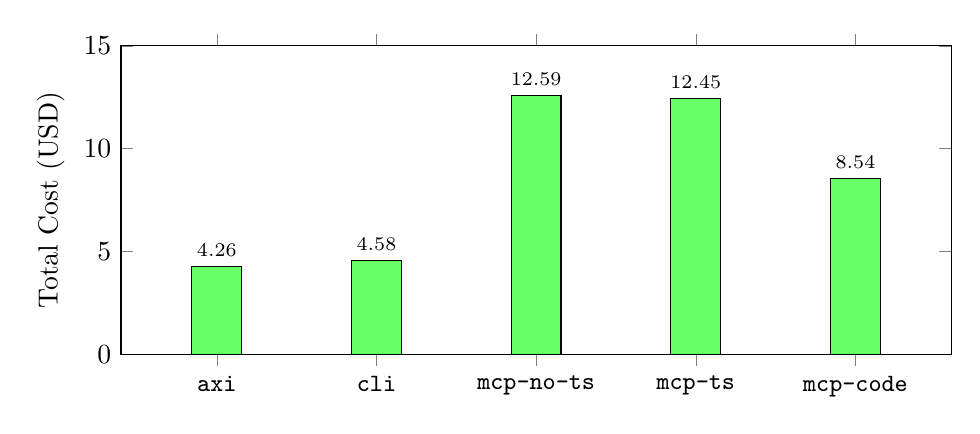
\begin{tikzpicture}
\begin{axis}[
    ybar,
    bar width=18pt,
    width=\columnwidth,
    height=5.5cm,
    ylabel={Total Cost (USD)},
    symbolic x coords={axi, cli, mcp-no-ts, mcp-ts, mcp-code},
    xtick=data,
    xticklabels={\texttt{axi}, \texttt{cli}, \texttt{mcp-no-ts}, \texttt{mcp-ts}, \texttt{mcp-code}},
    ymin=0, ymax=15,
    nodes near coords,
    nodes near coords align={vertical},
    every node near coord/.append style={font=\scriptsize},
    enlarge x limits=0.15,
    xticklabel style={font=\small},
]
\addplot[fill=green!60] coordinates {(axi,4.26) (cli,4.58) (mcp-no-ts,12.59) (mcp-ts,12.45) (mcp-code,8.54)};
\end{axis}
\end{tikzpicture}
\caption{Total cost across 85 runs per condition. AXI and CLI cost
\$4--5 total. MCP conditions cost \$8--13---a 2--3$\times$ premium driven
by schema overhead in the context window.}
\label{fig:cost}
\end{figure}

% ---------------------------------------------------------------------------
% 6  ANALYSIS
% ---------------------------------------------------------------------------
\section{Analysis}
\label{sec:analysis}

\subsection{Finding 1: AXI Achieves 100\% Reliability at Lowest Cost}

AXI is the only condition that passes all 85 runs (100\% success) at an
average cost of \$0.050/task---7\% less than CLI's \$0.054 and 66\% less than
the cheapest MCP condition (\$0.101 for \texttt{mcp-with-code-mode}). AXI also has the fastest
average duration (15.7s vs.\ 17.4s for CLI, 34--43s for MCP). The reliability
advantage is most pronounced on aggregate tasks (where pre-computed
\texttt{totalCount} fields eliminate pagination errors) and complex
investigations (where contextual suggestions prevent wrong turns).
Table~\ref{tab:pertask} shows the full per-task breakdown.

\subsection{Finding 2: MCP Conditions Are 2--3$\times$ More Expensive}

The MCP cost premium (Table~\ref{tab:pertask}) is not uniform---it
concentrates on complex tasks where schema overhead compounds across many
turns.
On \texttt{ci\_failure\_investigation}, \texttt{mcp-no-toolsearch} averages \$0.758/task
across 15 turns and 177 seconds, vs.\ AXI's \$0.065 across 3 turns and
21 seconds---a \textbf{12$\times$ cost difference}. The agent re-sends the
full tool schema catalog (176K tokens) on every turn; by turn 15, schema
tokens dominate the context.

On simple tasks where agents need few turns, MCP's overhead is more modest:
\texttt{view\_pr} costs \$0.045 for MCP vs.\ \$0.039 for AXI (1.2$\times$).

\subsection{Finding 3: ToolSearch Saves Upfront Tokens but Spends Them on Extra Turns}

ToolSearch starts with a smaller context ($\sim$50K vs.\ $\sim$83K tokens)
but needs 1--2 extra turns per task for tool discovery. Each extra turn
re-sends the growing conversation, so the savings are consumed by
accumulation. On \texttt{merged\_pr\_ci\_audit} (Table~\ref{tab:pertask}),
\texttt{mcp-with-toolsearch} takes 24 turns at \$0.614/task vs.\
\texttt{mcp-no-toolsearch}'s 18 turns at \$0.340---1.8$\times$ more
expensive and 2.2$\times$ slower, with identical success (3/5). ToolSearch also introduces a new failure mode: on
\texttt{run\_then\_jobs}, the agent cannot find the right tool via search
(0/5), while eager loading succeeds 4/5.

\subsection{Finding 4: \texttt{mcp-with-code-mode} Is Cheapest MCP but Still 2$\times$ AXI}

The \texttt{mcp-with-code-mode} condition, where the agent writes TypeScript
scripts calling typed wrapper functions, achieves the lowest cost among MCP
conditions (\$0.101/task). Writing code amortizes schema costs by batching
multiple API calls per script. But the code-generation overhead makes it the
\emph{slowest} condition (43.4s avg, the longest of all five). On
\texttt{ci\_failure\_investigation}, \texttt{mcp-with-code-mode} costs \$0.194/task---3$\times$
AXI's \$0.065---but achieves 5/5 success, outperforming both direct MCP
conditions (2/5 each). Code-mode also introduces a unique failure mode:
unhandled runtime errors cause 4/5 failures on \texttt{nonexistent\_repo},
where the agent writes scripts that throw instead of gracefully reporting
the error.

\subsection{Finding 5: AXI's Advantages by Task Type}

AXI's advantages vary by task complexity, not just success rate:

\paragraph{Simple lookups.}
All conditions achieve 100\% success. AXI and CLI cost \$0.024--0.039/task;
MCP costs \$0.031--0.100/task. The 1.5--3$\times$ MCP premium is pure schema
overhead.

\paragraph{Multi-step investigations.}
AXI and CLI both achieve 100\% success on most tasks. The cost difference
emerges on the hardest tasks: \texttt{ci\_failure\_investigation} costs
\$0.065 for AXI vs.\ \$0.061 for CLI (both 5/5), but \$0.194--0.758 for MCP
conditions (2--5/5). AXI's pre-computed job status fields
(\texttt{checks: "27 passed, 0 failed"}) eliminate the need for separate
job-listing API calls that MCP agents must make turn by turn.

\paragraph{Aggregate tasks.}
This is where AXI separates from all conditions. \texttt{list\_labels}:
AXI 5/5 at \$0.044; every other condition 0/5. \texttt{weekly\_catchup}:
AXI 5/5 at \$0.050; \texttt{cli} 0/5; \texttt{mcp-with-code-mode} 0/5. The pre-computed
\texttt{totalCount} field is the difference---without it, agents report
the default page size (30) as the total.

\paragraph{Error handling.}
All CLI-based conditions handle errors well. \texttt{mcp-with-code-mode} scores only 1/5 on
\texttt{nonexistent\_repo} (\$0.069/task) because generated scripts throw
unhandled exceptions rather than reporting structured errors.

\subsection{Case Study A: \texttt{ci\_failure\_investigation}}

This task asks the agent to identify the 5 most recent failed CI runs and
report which jobs failed in each. It is a multi-step investigation requiring
the agent to list runs, then drill into each one to inspect job-level results.

\begin{lstlisting}[caption={AXI: 3 turns, \$0.065, 21s (SUCCESS).},label=lst:axi-ci]
Turn 1 (agent -> tool):
$ gh-axi run list --status failure --limit 5

Turn 1 (tool -> agent):
runs[5]{id,title,status,conclusion,workflow,branch}:
  23386042824,"fix(daemon): repair stale LaunchAgent
    ...",completed,failure,Install Smoke,...
  23385977677,"feat(auth): add models auth clean
    ...",completed,failure,CI,...
  ... (3 more)
help[1]:
  Run `gh-axi run view <id>` to view details

Turn 2: Agent views all 5 runs in parallel

Turn 2 (tool -> agent, for each run):
run:
  id: 23385977677
  conclusion: failure
  workflow: CI
jobs[29]{name,status,conclusion}:
  check,completed,failure
  check-additional,completed,failure
  build-smoke,completed,failure
  ... (26 more with pass/skip/fail)
help[2]:
  Run `gh-axi run view 23385977677 --log-failed`
    to see failure logs

Turn 3: Agent summarizes patterns.
\end{lstlisting}

AXI completes in 3 turns. The key advantage: each \texttt{run view}
response includes the full job-level breakdown (\texttt{jobs[29]
\{name,status,conclusion\}}) as structured data, plus a suggestion to
view failure logs. The agent can immediately identify which jobs failed
without additional API calls.

\begin{lstlisting}[caption={\texttt{mcp-no-toolsearch}: 15 turns, \$0.758, 177s (FAIL 2/5).}]
Turn 1: list_workflow_runs(status:"failure",per_page:5)
  -> 5 run objects (~2KB JSON each)
Turn 2: list_workflow_run_jobs(run_id:23385977677)
  -> 29 job objects (~1.5KB JSON each)
  (context now: 176K schema + growing conversation)
Turn 3: list_workflow_run_jobs(run_id:23385977675)
  -> 2 job objects
Turn 4-6: ... (remaining runs)
  (context exceeding 400K tokens by turn 6)
Turn 7-15: Agent re-reads earlier results,
  attempts to correlate, loses track of which
  jobs belong to which run.
Result: 2/5 runs produce correct answer.
  3/5 runs misattribute job failures or omit runs.
\end{lstlisting}

MCP requires separate API calls for run listing and job listing (no
inline job status). Each call re-sends the full schema catalog.
By turn 6, the context exceeds 400K tokens, and the agent begins
confusing job data across runs.

\subsection{Case Study B: \texttt{merged\_pr\_ci\_audit}}

This task asks the agent to list the 10 most recently merged PRs and
report the CI status of each. It tests whether the interface provides
efficient access to both PR metadata and CI results.

\begin{lstlisting}[caption={AXI: 5 turns, \$0.064, 26s (SUCCESS 5/5).}]
Turn 1: $ gh-axi pr list --state merged --limit 10
  -> count: 10 of 3549 total
     pull_requests[10]{number,title,state,...}:
       51772,"refactor(plugins): route Telegram..."
       ...
     help: Run `gh-axi pr view <number>`

Turns 2-5: View each PR (some in parallel)
  -> checks: "27 passed, 0 failed, 10 skipped"
     (pre-computed -- no extra API call needed)

Agent summarizes: "6 out of 10 fully green CI."
\end{lstlisting}

The key: AXI's pre-computed \texttt{checks} field provides a one-line CI
summary inline in each PR view. The agent never needs to call a separate
checks or workflow API.

\begin{lstlisting}[caption={CLI: 4 turns, \$0.076, 42s (SUCCESS 5/5).}]
Turn 1: $ gh pr list --state merged --limit 10
          --json number,title,author,mergedAt,
                 statusCheckRollup
  -> 10 PR objects with nested check arrays
     (~2KB JSON each)
  Agent must know the --json field name
  "statusCheckRollup"

Turns 2-3: Parse JSON, count pass/fail per PR.
  Some runs call `gh pr checks` again to
  double-check results -- redundant work.

Turn 4: Agent summarizes results.
\end{lstlisting}

CLI also succeeds (5/5) by using the \texttt{-{}-json} flag to get
structured output in a single call. However, CLI costs 19\% more
(\$0.076 vs.\ \$0.064) and takes 62\% longer (42s vs.\ 26s).
The CLI agent must know to use \texttt{-{}-json} with
\texttt{statusCheckRollup}---a non-obvious field name that requires
prior knowledge of the \texttt{gh} CLI's JSON schema. In some runs,
the agent hedges by calling \texttt{gh pr checks} separately to
verify the JSON data, adding redundant API calls.

\begin{lstlisting}[caption={\texttt{mcp-with-toolsearch}: 24 turns, \$0.614, 136s (FAIL 3/5).}]
Turns 1-3: ToolSearch for PR listing tool
Turns 4-6: List merged PRs, paginate
Turns 7-24: For each PR, search for check/status
  tool, invoke it, parse response.
  Context grows to >300K tokens.
  Agent loses track of PR-to-check mapping.
Result: 3/5 runs succeed. 2/5 misreport CI status.
\end{lstlisting}

\texttt{mcp-with-toolsearch} takes 24 turns, costs 9.6$\times$ more than AXI, and still
fails 40\% of the time. The combination of tool discovery overhead and
the need for separate check-fetching calls compounds across 10 PRs.

% ---------------------------------------------------------------------------
% 7  LIMITATIONS
% ---------------------------------------------------------------------------
\section{Limitations}
\label{sec:limitations}

\begin{itemize}
  \item \textbf{Single target repository.} All tasks target
    \texttt{openclaw/openclaw}. Results may vary on repositories with
    different sizes or structures.
  \item \textbf{Single agent model.} Only Claude Sonnet~4.6 is evaluated.
    Other models may exhibit different sensitivities to output format.
  \item \textbf{Read-only tasks.} The benchmark includes only read operations.
    Mutations introduce additional challenges around idempotency.
  \item \textbf{LLM judge.} Task success is determined by an LLM judge,
    which may introduce scoring biases.
  \item \textbf{GitHub-specific implementation.} While the AXI principles
    are domain-general, this evaluation is specific to GitHub.
  \item \textbf{Auto-generated MCP baseline.} The MCP conditions use the
    official GitHub MCP server, not a hand-optimized one. A carefully designed
    MCP server with fewer, better-composed tools could narrow the gap.
\end{itemize}

% ---------------------------------------------------------------------------
% 8  CONCLUSION
% ---------------------------------------------------------------------------
\section{Conclusion}
\label{sec:conclusion}

The debate between CLI and MCP as agent-tool interfaces misses the deeper
question: what design principles make any interface effective for agents?
This evaluation shows that a principled CLI design (AXI) outperforms both
raw CLI and MCP on every metric---success, cost, duration, and turns.

AXI achieves 100\% reliability at \$0.050/task, compared to 86\% at
\$0.054 for raw CLI and 82--87\% at \$0.101--0.148 for MCP. The cost gap
widens dramatically on complex tasks: \texttt{ci\_failure\_investigation}
costs \$0.065 for AXI vs.\ \$0.758 for MCP (12$\times$), with AXI achieving
100\% success vs.\ MCP's 40\%.

The key principles are: (1) pre-computed fields like \texttt{totalCount} and
CI status summaries eliminate entire classes of agent errors and unnecessary
API calls; (2) token-efficient output keeps context budgets available for
reasoning rather than parsing; and (3) contextual suggestions guide agents
through multi-step workflows without requiring prior knowledge of the tool's
API surface.

These principles are transport-agnostic. They apply whether the underlying
mechanism is a CLI, an MCP server, or a typed SDK. The 10 AXI principles
provide a concrete, testable framework for designing agent-tool interfaces
that are both reliable and cost-efficient.

% ---------------------------------------------------------------------------
% REFERENCES
% ---------------------------------------------------------------------------

\begin{thebibliography}{4}

\bibitem{mcp2024}
Anthropic.
\newblock Model Context Protocol specification.
\newblock Technical report, Anthropic, 2024.
\newblock \url{https://modelcontextprotocol.io}.

\bibitem{smithery2026}
H.~Mao and R.~Pradhan.
\newblock MCP vs CLI is the wrong fight.
\newblock Smithery Blog, March 2026.
\newblock \url{https://smithery.ai/blog/mcp-vs-cli-is-the-wrong-fight}.

\bibitem{anthropic2025code}
A.~Jones and C.~Kelly.
\newblock Code execution with MCP: Building more efficient agents.
\newblock Anthropic Engineering Blog, November 2025.
\newblock \url{https://www.anthropic.com/engineering/code-execution-with-mcp}.

\bibitem{cloudflare2025code}
K.~Varda and S.~Pai.
\newblock Code Mode: The better way to use MCP.
\newblock Cloudflare Blog, September 2025.
\newblock \url{https://blog.cloudflare.com/code-mode/}.

\end{thebibliography}

\end{document}
